\documentclass[tikz, border=1cm]{standalone}
\usetikzlibrary{bbox}
\begin{document}
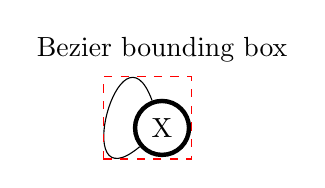
\begin{tikzpicture}[bezier bounding box]
\node[circle, draw, ultra thick] (activity) {X};
\draw (activity) to[out=110, in=220, min distance=0.25cm, looseness=5] (activity);
\draw[red, dashed] (current bounding box.south west) rectangle (current bounding box.north east);
\node at (0,1) {Bezier bounding box};
\end{tikzpicture}
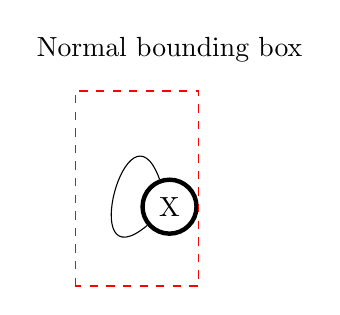
\begin{tikzpicture}
\node[circle, draw, ultra thick] (activity) {X};
\draw (activity) to[out=110, in=220, min distance=0.25cm, looseness=5] (activity);
\draw[red, dashed] (current bounding box.south west) rectangle (current bounding box.north east);
\node at (0,2) {Normal bounding box};
\end{tikzpicture}
\end{document}